\documentclass[fleqn]{exam}

\usepackage{fullpage}
\usepackage{enumerate}
\usepackage{unitsdef} 
\usepackage{graphicx}
\usepackage[fleqn]{mathtools}
\usepackage{cancel}
\usepackage{polynom}
\usepackage{float}
\usepackage{mdwlist}
\usepackage{booktabs}
\usepackage{cancel}
\usepackage{polynom}
\usepackage{caption}

\setlength{\mathindent}{.5 cm}

\everymath{\displaystyle}

% \begin{figure}[H]
%   \centering
%   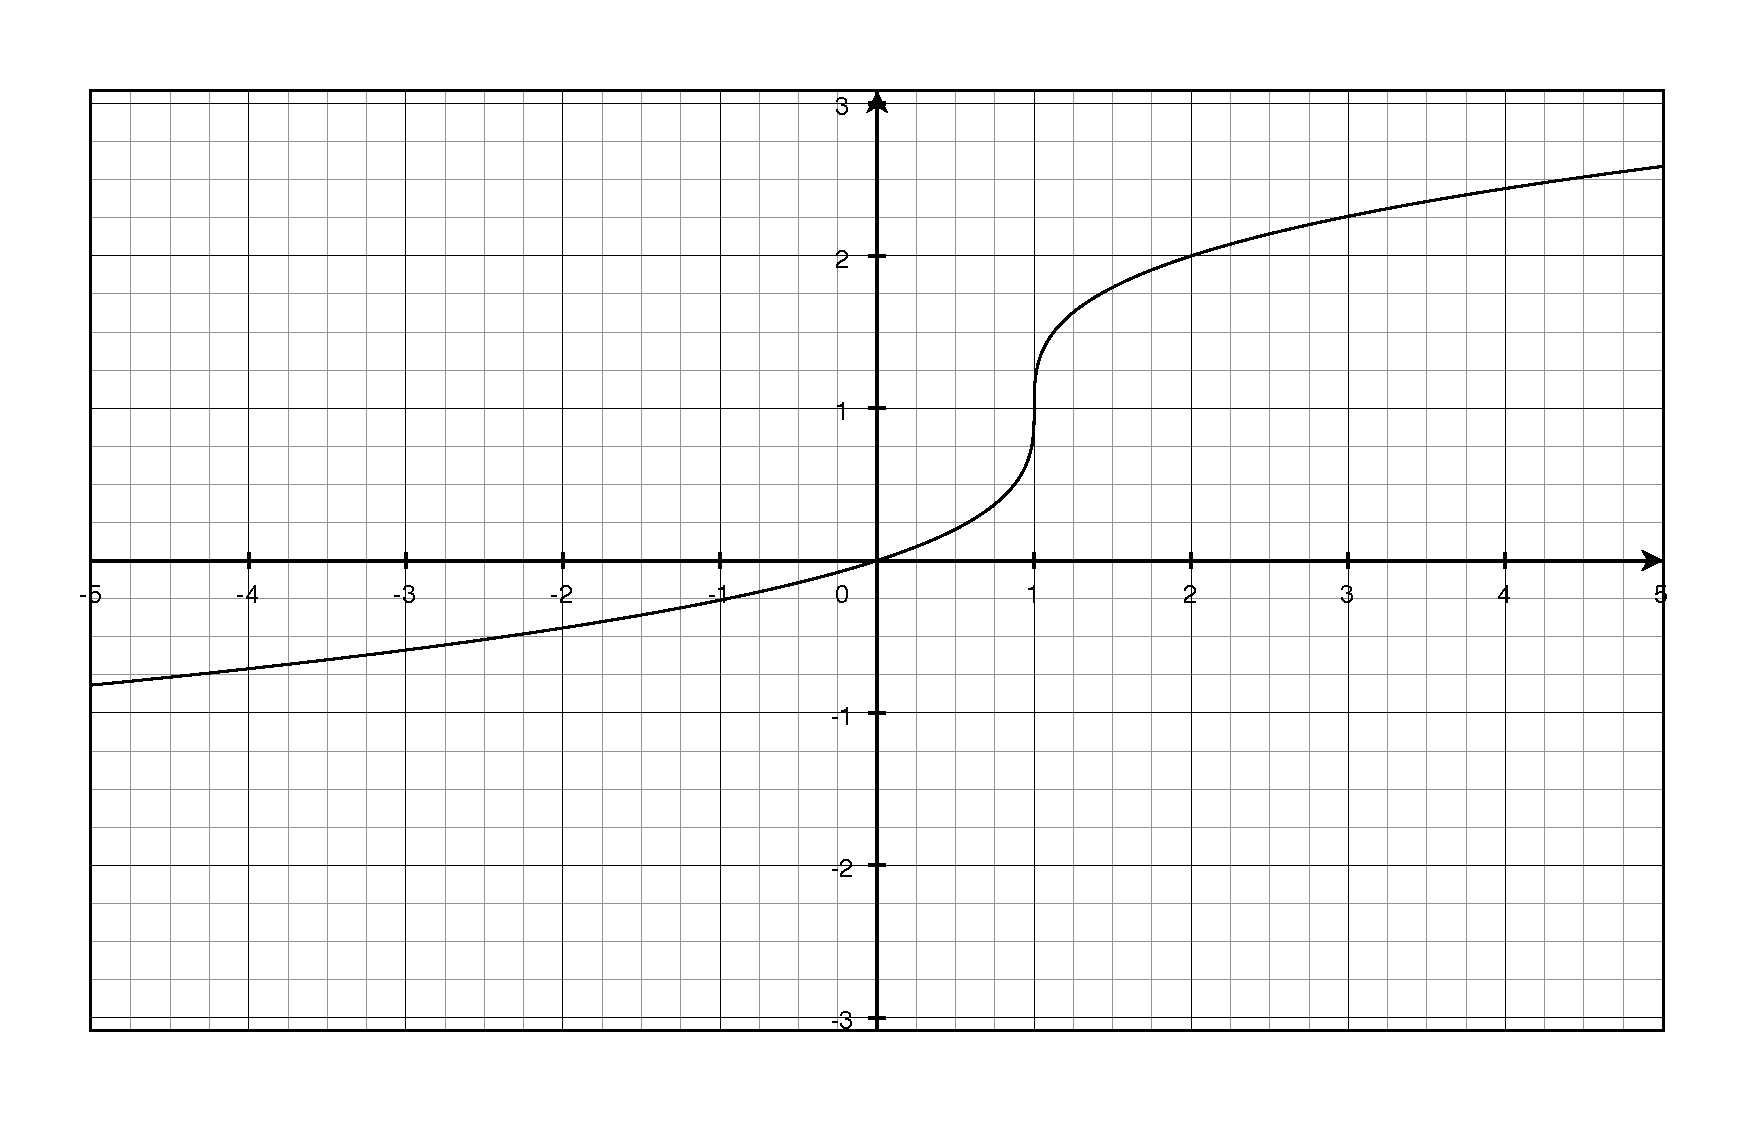
\includegraphics[scale=.3]{question7.eps}
%   \caption*{Question 7}
% \end{figure}

% \begin{tabular}{cc}
% \toprule
% period & amplitude \\
% \midrule
%   $\pi$ & $2$ \\
% \bottomrule
% \end{tabular}

\newunit{\inch}{in}
\newunit{\mile}{mile}
\newunit{\foot}{ft}
\newunit{\knot}{knot}
\newunit{\gallon}{gallon}

\printanswers

\ifprintanswers 
\usepackage{2in1, lscape} 
\fi

\title{Math 263A \\ Homework 12}
\date{April 25, 2012}

\begin{document}

\maketitle

\section{Homework}

\begin{itemize*}
  \item Read Section 4.1
  \item pp. 180-182: 1-10, 12, 15, 19-20, 23-24, 27
\end{itemize*}

\section{Extra Credit}
Page 180-181, problem 22 and 28

\ifprintanswers

\pagebreak

\begin{description}

\item[22]
If $L$ is the length of the wire and $x$ is the amount of wire used for the circle, the radius of the circle is:

\begin{align*}
  x &= 2 \pi r \\
  r &= \frac{x}{2 \pi} \\
\end{align*}
The area of the circle is:
\begin{align*}
  A_{circle} &= \pi r^2 \\
    &= \pi \cdot \left( \frac{x}{2 \pi} \right)^2 \\
    &= \frac{x^2}{4 \pi} \\
\end{align*}

The rest of the wire is used for the square, so the area from the square is: 
\[
  A_{square} = \left( \frac{L - x}{4} \right)^2
\]

For a wire of length $L$, the total area is:
\[
  A_{total} = \frac{x^2}{4 \pi} + \left( \frac{L - x}{4} \right)^2
\]

To find the minimum and maximum areas, we need to find the points where the derivative of the area is zero:
\begin{align*}
  A' &= \frac{x}{2 \pi} + 2 \cdot \left( \frac{L - x}{4} \right) \cdot \left( -\frac{1}{4} \right) \\
     &= \frac{x}{2 \pi} + \frac{x - L}{8} \\
\\
  \frac{x}{2 \pi} + \frac{x - L}{8} &= 0 \\
  4x + \pi x - \pi L &= 0 \\
  x &= \frac{\pi L}{\pi + 4} \\
\end{align*}

For this problem, $L = 16$ and the critical points are $x = \{0, 7.0384, 16\}$

\begin{align*}
  A(0) &= 16 \\
  A(7.0384) &\approx 8.9616 \\
  A(16) &\approx 20.3718 \\ 
\end{align*}

The best thing to do is bend the whole wire into a circle which gives you a total area of $20.3718 \inch^2$.  

The worst thing to do is to split the wire approximately in half, making a circle with circumference 7.0384 inches and a
total area of $8.9616 \inch^2$.

\pagebreak

\item[28]

From the picture, $y = \sqrt{r^2 - x^2}$

First find a formula for the area:
\begin{align*}
  A &= 2xy \\
      &= 2x \sqrt{r^2 - x^2} \\
      &= 2 \sqrt{r^2x^2 - x^4} \\
\end{align*}

differentiate:
\begin{align*}
  A' &= 2 \cdot \frac{1}{2}(r^2x^2 - x^4)^{-1/2}(2r^2x - 4x^3) \\
     &= \frac{2r^2x - 4x^3}{\sqrt{r^2x^2 - x^4}} \\
\end{align*}

set the derivative to zero to find the maximum.  We can ignore the solution where $x=0$, since this certainly won't be a maximum:
\begin{align*}
  2r^2x - 4x^3 &= 0 \\
  % r^2x - 2x^3 &= 0 \\
  x(r^2 - 2x^2) &= 0 \\
  r^2 - 2x^2 &= 0 \\
  x &= \frac{r}{\sqrt{2}} \\
\end{align*}

The y-dimension is:
\[
  y = \sqrt{r^2 - x^2} = \sqrt{r^2 - \frac{r^2}{2}} = \frac{r}{\sqrt{2}} 
\]

So the rectangle should have $x$ and $y$ both $\frac{r}{\sqrt{2}}$.

\pagebreak

\uplevel{\section{Homework}}

\item[1]
$f(x) = x^2 + 4x + 4$, $I = [-4, 0]$

\begin{align*}
  f'(x) &= 2x + 4 \\
  2x + 4 &= 0 \\
  x &= -2 \\
\end{align*}

The critical points are $x = \{-4, -2, 0 \}$:

\begin{tabular}{rrr}
\toprule
x   & f(x) & \\
\midrule
$-4$  &   4  & max \\
$-2$  &   0  & min \\
0     &   4  & max \\
\bottomrule
\end{tabular}

\item[2]
$f(x) = x^2 + x$, $I = [-2, 2]$

\begin{align*}
  f'(x) &=  2x + 1 \\
  2x + 1 &= 0 \\
  x &= - \frac{1}{2}
\end{align*}

The critical points are $x = \left\{ -2, - \frac{1}{2}, 2 \right\}$:

\begin{tabular}{rrr}
\toprule
x   & f(x) & note \\
\midrule
$-2$    &   2       &  \\
$-0.5$  &  $-0.25$  & min \\
2       &   6       & max \\
\bottomrule
\end{tabular}

\pagebreak
\item[3]
$f(x) = x^2 + 3x$, $I = [-2, 1]$

\begin{align*}
  f'(x) &= 2x + 2 \\
  2x + 3 &= 0 \\
  x &= - \frac{3}{2} \\
\end{align*}

The critical points are $x = \left\{-2, -\frac{3}{2}, 1 \right\}$:

\begin{tabular}{rrr}
\toprule
x   & f(x) & note \\
\midrule
$-2$    &  $-2$    &  \\
$-3/2$  &  $-9/4$  & min \\
1       &   4      & max \\
\bottomrule
\end{tabular}

\item[4]
$G(x) = \frac{1}{5}(2x^3 + 3x^2 - 12x)$, $I = [-3, 3]$

\begin{align*}
  G'(x) &= \frac{1}{5}(6x^2 + 6x - 12) \\
  6x^2 + 6x - 12 &= 0 \\
  x^2 + x - 2 &= 0 \\
  (x + 2)(x - 1) &= 0 \\
  x &= \{-2, 1\}
\end{align*}

The critical points are $x = \{-3, -2, 1, 3 \}$:

\begin{tabular}{rrr}
\toprule
x   & f(x) & note \\
\midrule
$-3$            &  $1.8$        &  \\
$-2$            &  $4$          &   \\
$1$             &  $-1.4$       &  min \\
$3$             &  $9$          &  max \\
\bottomrule
\end{tabular}

\pagebreak

\item[5] 
$f(x) = x^3 - 3x + 1$, $I = \left(-\frac{3}{2}, 3 \right)$

\begin{align*}
  f'(x) &= 3x^2 - 3 \\
  3x^2 - 3 &= 0 \\
  x^2 - 1  &= 0 \\
  (x + 1)(x - 1) &= 0 \\
  x &= \{-1, 1\}
\end{align*}

The critical points are $x = \{ -1, 1 \}$:

\begin{tabular}{rrr}
\toprule
x   & f(x) & note \\
\midrule
$-1.5$ &  $2.125$ &  \\
$-1$   &  $3$     &  \\
$1$    &  $-1$    &   min \\
$3$    &  $19$    &   \\
\bottomrule
\end{tabular}

There is no maximum because the endpoints aren't included.

\item[6]
This is just like number 5 except the endpoints are included.  So in this case the maximum is $(3, 19)$.

\item[7] $h(r) = \frac{1}{r}$, $I = [-1, 3]$

%% \begin{align*}
%%   h'(r) &= - \frac{1}{r^2} \\
%% \end{align*}

%% The critical points are $x = \{-1, 3\}$
%% \begin{align*}
%%   f(-1) &=  -1 \\
%%   f(3)  &=  \frac{1}{3}\\
%% \end{align*}

There is no minimum or maximum because the graph approaches $\pm \infty$ around zero which is included in the interval.

\item[8] $g(x) = \frac{1}{1+x^2}$; $I = [-3, 1]$
\begin{align*}
  g'(x) &= -\frac{2x}{(1 + x^2)^2} \\ 
  2x &= 0 \\
  x  &= 0 \\
\end{align*}

The critical points are $x = \{-3, 0, 1\}$

\begin{tabular}{rrr}
\toprule
x   & f(x) & note \\
\midrule
$-3$            &  $0.1$        &  min \\
$0$            &  $1$           &  max \\
$1$            &  $0.5$          &   \\
\bottomrule
\end{tabular}

\item[9]
$g(x) = \frac{1}{1+x^2}$; $I = (- \infty, \infty)$

\begin{itemize*}
  \item $g$ is always positive, but as $x$ approaches $\pm \infty$, $g(x)$ approaches $0$ but never actually gets there, so there
  is no minimum.
  \item the maximum is still $(0, 1)$.
\end{itemize*}

\item[10] 
$f(x) = \frac{x}{1+x^2}$; $I = [-1, 4]$

\begin{align*}
  g'(x) &= \frac{1+x^2 - x(2x)}{(1 + x^2)^2} \\ 
        &= \frac{1 - x^2}{(1 + x^2)^2} \\ 
  1 - x^2 &= 0 \\
  x  &= \pm 1 \\
\end{align*}

The critical points are $x = \{-1, 1, 4 \}$

\begin{tabular}{rrr}
\toprule
x   & f(x) & note \\
\midrule
$-1$ &  $-0.5$   &  min \\
$1$  &  $0.5$    &  max \\
$4$  &  $0.2353$ &   \\
\bottomrule
\end{tabular}


\item[12] 
$s(t) = \sin t - \cos t$; $I = [0, \pi]$
\begin{align*}
  s'(t) &= \cos t + \sin t \\
  \cos t + \sin t &= 0 \\
  \sin t &= -\cos t \\
  t &= \frac{3\pi}{4}
\end{align*}

The critical points are $x = \left\{0, \frac{3\pi}{4}, \pi \right \}$

\begin{tabular}{rrr}
\toprule
x   & f(x) & note \\
\midrule
$0$               &  $-1$       &  min \\
$3\pi/4$  &  $\sqrt{2}$    &  max \\
$\pi$             &  $1$ &   \\
\bottomrule
\end{tabular}

\item[15] 
$g(t) = \sqrt[3]{x}$; $I = [-1, 27]$
\begin{align*}
  g'(x) &= \frac{1}{3} x^{-2/3} \\
\end{align*}

$g'$ is undefined at $x = 0$, so the critical points are $x = \{-1, 0, 27\}$

\begin{tabular}{rrr}
\toprule
x   & f(x) & note \\
\midrule
$-1$ & $-1$ & min \\
$0$  & $0$  &     \\
$27$ & $3$  & max \\
\bottomrule
\end{tabular}

\item[19]
\begin{align*}
  2x + 2y &= 200 \\
  x + y &= 100 \\
  y &= 100 - x \\
\\
  A &= xy \\
    &= (100 - x) x \\
    &= 100x - x^2 \\
\\
  A' &= 100 - 2x \\
  100 - 2x &= 0 \\
  x &= 50 \\
\\
  y &= 100 - 50 = 50 \\
\end{align*}

She should make a square yard with each side 50 feet long.

\item[20]
\begin{align*}
  K &= 2x + 2y \\
  2y &= K - 2x \\
  y  &= \frac{K}{2} - x \\
\\
  A &= xy \\
    &= \left(\frac{K}{2} - x \right) x \\
    &= \frac{Kx}{2} - x^2 \\
\\
  A' &= \frac{K}{2} - 2x \\
  \frac{K}{2} - 2x &= 0 \\
  x &= \frac{K}{4} \\
\\
  y &= \frac{K}{2} - \frac{K}{4} = \frac{K}{4} \\
\end{align*}

\item[23]
\begin{align*}
  P &= 2x + y \\
  y &= P - 2x \\
\\
  A &= xy \\
    &= x(P - 2x) \\
    &= Px - 2x^2 \\
\\
  A' &= P - 4x \\
  P - 4x &= 0 \\
  x &= \frac{P}{4} \\
  y &= \frac{P}{2} \\
\end{align*}

$x = 20$ and $y = 40$


\item[24]
\begin{align*}
  P &= 4x + y \\
  y &= P - 4x \\
\\
  A &= xy \\
    &= x(P - 4x) \\
    &= Px - 4x^2 \\
\\
  A' &= P - 8x \\
  P - 8x &= 0 \\
  x &= \frac{P}{8} \\
  y &= \frac{P}{2} \\
\end{align*}

$x = 10$ and $y = 40$

\item[27]
The width of the rectangle is $2x$ and the height is $12 - x^2$, so the area is $2x(12 - x^2)$.
\begin{align*}
  A &= 2xy \\
    &= 2x(12-x^2) \\
    &= 24x - 2x^3 \\
\\
  A' &= 24 - 6x^2 \\
\\
  24 - 6x^2 &= 0 \\
  4 - x^2 &= 0 \\
  x &= \pm 2 \\
\end{align*}

The maximum area of 32 occurs when $x = 2$ and $y = 8$.

\end{description}

\else

\vspace{10 cm}

{\em When we are unhurried and wise, we perceive that only great and worthy things have any permanent and absolute
existence,---that petty fears and petty pleasures are but the shadow of reality.}

\vspace{.2 cm}

\hspace{1 cm} --Henry David Thoreau

\fi

\end{document}

